\paragraph{Theorem}
Chebychev inequality allows to find an estimate of the area between the
values $\mu-k\sigma\text{ and }\mu+k\sigma$ for some given $k\neq 0$, showing
that the area under $f(x)$ on the interval $\left[\mu-k\sigma, \mu+k\sigma
\right]$ is at least $1-k^{2}$.\\
Let $X$ be a random variable with probability density function $f(x)$. If
$\mu$ and $\sigma>0$ are the mean and standard deviation of $X$ then:
\begin{center}
	\enc{$\Prob{|X-\mu|<k\sigma}\geq 1-\frac{1}{k^{2}}$}
\end{center}
\begin{figure}[H]
	\begin{center}
		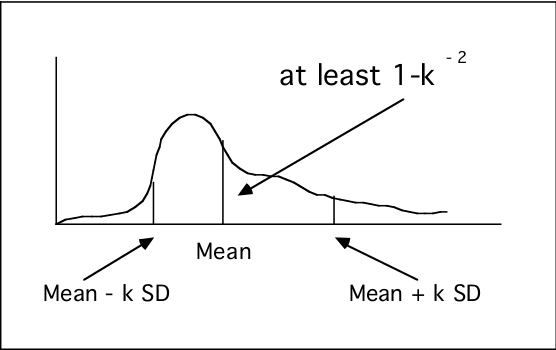
\includegraphics[width=\textwidth]{./chaps/13sec/4images/1IneqCheby.png}
	\end{center}
	\caption{Illustration of Chebychev inequality}
	\label{fig:fig2}
\end{figure}
